\documentclass{beamer}
\usetheme{Ilmenau}
\usecolortheme{default}
\usefonttheme{serif}

\usepackage{lipsum}
\usepackage{graphicx,xcolor,tikz,pgfplots}
\pgfplotsset{compat=1.14}
\usepackage{amsmath,amssymb,amsfonts}
\usetikzlibrary[automata] % ConTEXt
\usepackage{rotating}
\usepackage[export]{adjustbox}
\usepackage{relsize}
\tikzset{fontscale/.style = {font=\relsize{#1}}
    }

\newtheorem{thm}{Theorem}
\newtheorem{dfn}{Definition}

\newcommand{\ds}{\displaystyle}
\newcommand{\R}{{\mathbb R}}
\newcommand{\Q}{{\mathbb Q}}
\newcommand{\Z}{{\mathbb Z}}
\newcommand{\N}{{\mathbb N}}
\newcommand{\C}{{\mathbb C}}
\DeclareMathOperator{\Ap}{Ap}
\DeclareMathOperator{\PF}{PF}
\DeclareMathOperator{\KC}{KC}
\DeclareMathOperator{\ewt}{ewt}
\DeclareMathOperator{\wt}{wt}
\DeclareMathOperator{\Apwt}{Apwt}

\setbeamertemplate{footline}[frame number]{}
\setbeamertemplate{navigation symbols}{}

\defbeamertemplate*{headline}{split theme}
{}


\title{Pflueger's Conjecture for Numerical Semigroups of Small Depths\\[5pt]\footnotesize{\textit{JMM 2025}}}
\author{Ian Farish, Erik Imathiu-Jones, Kaylee Seojin Lee Kim, Max LaFortune, Cole McGeorge, \textbf{Victoria Wiest}
\\[15pt] Graduate Student Advisors: Fabian Ramirez, Deepesh Singhal
\\[15pt] Faculty Advisor: Dr. Nathan Kaplan}
\institute{}
\date{}

\begin{document}

\begin{frame}
\titlepage
\end{frame}

\section{Preliminaries}
\begin{frame}{Numerical Semigroups}
    A nonempty subset of $\N_{0}=\{0,1,2,3,\dots\}$, denoted as $S$, is a \textbf{numerical semigroup}, if and only if

    \begin{itemize}
        \item $0\in S$,
        \item $\N_{0} - S$ is finite, and
        \item If $x\in S$ and $y\in S$, then $x+y\in S$ (closed under addition)
    \end{itemize}\vspace{8pt}
    Ex: $\{0,3,4,6,7,8,\to\}$
    
\end{frame}

\begin{frame}{Definitions related to Numerical Semigroups}
    The smallest nonzero element in $S$ is called the \textbf{multiplicity}, denoted by $m(S)$.\\[15pt]
    
    We refer to $\N_{0} - S$ as the set of gaps in the numerical semigroup. 
    \begin{itemize}
        \item The number of gaps of a numerical semigroup is called the \textbf{genus}, denoted as $g(S).$
        \item The \textbf{Frobenius number}, $F(S)$, of a numerical semigroup is the largest gap.
    \end{itemize}
    \vspace{15pt}
    The \textbf{depth} of a numerical semigroup $S$ is the natural number $d$ such that 
    \[(d-1)m<F<dm.\]
\end{frame}

\begin{frame}{Minimal Generators}
    Every numerical semigroup, $S$, has a unique \textbf{minimal generating set} that generates $S$ by taking all possible nonnegative linear combinations of the numbers in the minimal generating set i.e., 
    \[\langle3,4\rangle=\{0,3,4,3+3,3+4,4+4,\to\}=\{0,3,4,6,7,8,\to\}\]\\[15pt]
    
    We refer to the elements in the minimal generating set as \textbf{minimal generators}.
\end{frame}

\begin{frame}{Young Diagram associated to a NS}
Every numerical semigroup is associated to some Young Diagram where \textbf{every element in $S$ is represented as a right step} ($\rightarrow$) and \textbf{every gap is represented as an up step} ($\uparrow$).\\[15pt]

    Ex: $\langle 3,8,10\rangle=\{0,3,6,8,9,10,\to\}$

        \begin{center}
            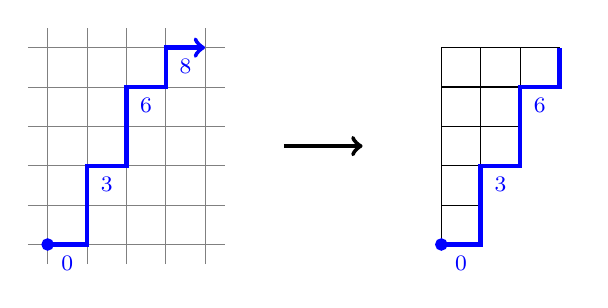
\begin{tikzpicture}[scale = .5]
		
			% 1 - rim lines
			\begin{scope}
				\draw[help lines] (-.5,-.5) grid (4.5,5.5);
				
				\begin{scope}[blue, ultra thick]
					\filldraw (0,0) circle [radius = 0.1];
					\draw[->, font = \footnotesize]
						(0,0) --
						node [below] {$0$} ++(1,0) --
						node [right] {} ++(0,1) -- 
						node [right] {} ++(0,1) --
						node [below] {$3$} ++(1,0) --
						node [right] {} ++(0,1) --
						node [right] {} ++(0,1) --
						node [below] {$6$} ++(1,0) --
						node [right] {} ++(0,1) --
						node [below] {$8$} ++(1,0);
				\end{scope}
			\end{scope}
		
			% 2 - rim with Young diagram and hooks
			\begin{scope}[xshift = 10cm]
                \foreach \x in {0,1,2}
					{ \draw (\x,4) rectangle ++(1,1);}
                \foreach \x in {0,1}
					{ \draw (\x,3) rectangle ++(1,1);}
				\foreach \x in {0,1}
					{ \draw (\x,2) rectangle ++(1,1);}
				\foreach \x in {0}
					{ \draw (\x,1) rectangle ++(1,1);}
				\foreach \x in {0}
					{ \draw (\x,0) rectangle ++(1,1);}
				
				\begin{scope}[blue, ultra thick]
					\filldraw (0,0) circle [radius = 0.1];
					\draw[font = \footnotesize]
						(0,0) --
						node [below] {$0$} ++(1,0) --
						node [right] {} ++(0,1) -- 
						node [right] {} ++(0,1) --
						node [below] {$3$} ++(1,0) --
						node [right] {} ++(0,1) --
						node [right] {} ++(0,1) --
						node [below] {$6$} ++(1,0) --
      					node [right] {} ++(0,1);
				\end{scope}
			\end{scope}
			
			
			% arrows
			\begin{scope}[ultra thick,  black, ->]
				\draw (6,2.5) -- (8,2.5);
				%\draw (13,2.5) -- (15,2.5);
			\end{scope}
		\end{tikzpicture}
        \end{center}    
\end{frame}

\begin{frame}{Weight}
    The \textbf{weight} of a numerical semigroup $S$, denoted by $\wt(S)$, is
    \[\sum_{x\in S} \#\{\text{gaps above}\; x\}\quad\text{where}\; x>0\]

    Ex: $\langle3,8,10\rangle=\{0,3,6,8,\to\}$
    \begin{center}
        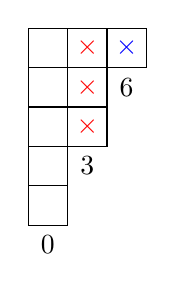
\begin{tikzpicture}[scale=0.5]
            \begin{scope}[xshift = 16cm]
                \foreach \x in {0,1,2}
					{ \draw (\x,4) rectangle ++(1,1);}
                \foreach \x in {0,1}
					{ \draw (\x,3) rectangle ++(1,1);}
				\foreach \x in {0,1}
					{ \draw (\x,2) rectangle ++(1,1);}
				\foreach \x in {0}
					{ \draw (\x,1) rectangle ++(1,1);}
				\foreach \x in {0}
					{ \draw (\x,0) rectangle ++(1,1);}
            \begin{scope}
                    \node at (0.5,-0.5) {$0$};
					\node at (1.5,1.5) {$3$};
					\node at (2.5,3.5) {$6$};
			\end{scope}
            \begin{scope}[red]
				\node at (1.5,2.5) {$\times$};
    			\node at (1.5,3.5) {$\times$};
				\node at (1.5,4.5) {$\times$};

            \end{scope}
            \begin{scope}[blue]
                \node at (2.5,4.5) {$\times$};
            \end{scope}
   		\end{scope}

        \end{tikzpicture}
    \end{center}
    \[\wt=4\]

\end{frame}

\begin{frame}{Upper Bound of Weight}
    \[S=\langle 2,2g+1\rangle\]

    \hfill

    \begin{center}
        \begin{tikzpicture}[scale=2]
            \coordinate (A) at (0,0);
            \coordinate (B) at (0.5,0);
            \coordinate (C) at (0.5,0.5);
            \coordinate (D) at (1,0.5);
            \coordinate (E) at (1,1);
            \coordinate (F) at (1.5,1);
            \coordinate (G) at (1.5,1.5);
            \coordinate (H) at (2,1.5);
            \coordinate (I) at (2,2);
            \coordinate (J) at (2.5,2);
            \coordinate (K) at (2.5,2.5);
            \coordinate (L) at (0,2.5);
            \coordinate (M) at (0.5,2.5);
            

            \draw (A) -- (B);
            \draw (B) -- (C);
            \draw (C) -- (D);
            \draw (D) -- (E);
            \draw (E) -- (F);
            \draw (F) -- (G);
            \draw (G) -- (H);
            \draw (H) -- (I);
            \draw (I) -- (J);
            \draw (J) -- (K);
            \draw (K) -- (L);
            \draw (L) -- (A);
            \draw (M) -- (B);

            \draw[decorate,decoration={brace,amplitude=3mm, raise=0.5mm}] (A) -- (L);

            \node at (-0.4,1.25) {$g$};
            \node at (1.15,1.7) [fontscale=3.45] {$\frac{g(g-1)}{2}$};
            \node at (0.25,-0.15) {$0$};
            \node at (0.75,0.35) {$2$};
        \end{tikzpicture}
        \end{center}    
\end{frame}

\begin{frame}{Effective Weight}
    Similar to the weight of a numerical semigroup, the \textbf{effective weight} of a numerical semigroup $S$, denoted by $\ewt(S)$, is
    \[\sum_{x\in S} \#\{\text{gaps above}\; x\}\quad\text{where}\; x\;\text{is a minimal generator}\]

    Ex: $\langle3,8,10\rangle=\{0,3,6,8,\to\}$    

    \begin{center}
        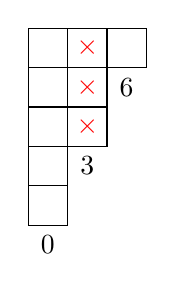
\begin{tikzpicture}[scale=0.5]
            \begin{scope}[xshift = 16cm]
                \foreach \x in {0,1,2}
					{ \draw (\x,4) rectangle ++(1,1);}
                \foreach \x in {0,1}
					{ \draw (\x,3) rectangle ++(1,1);}
				\foreach \x in {0,1}
					{ \draw (\x,2) rectangle ++(1,1);}
				\foreach \x in {0}
					{ \draw (\x,1) rectangle ++(1,1);}
				\foreach \x in {0}
					{ \draw (\x,0) rectangle ++(1,1);}
            \begin{scope}
                    \node at (0.5,-0.5) {$0$};
					\node at (1.5,1.5) {$3$};
					\node at (2.5,3.5) {$6$};
			\end{scope}
            \begin{scope}[red]
				\node at (1.5,2.5) {$\times$};
    			\node at (1.5,3.5) {$\times$};
				\node at (1.5,4.5) {$\times$};

            \end{scope}
   		\end{scope}

        \end{tikzpicture}
    \end{center}
    
    \[\ewt=3\]
\end{frame}

\begin{frame}{Pflueger's Conjecture}
    Analogously to the upper bound of $\wt(S)$, Nathan Plueger [1] has conjectured the following upper bound of $\ewt(S)$:
  \[\ewt(S)\leq\left\lfloor\frac{(g+1)^2}{8} \right\rfloor\]

  But unlike the upper bound of $\wt(S)$, Pflueger's upper bound has not been proven.
\end{frame}

\begin{frame}{Pflueger's Conjecture for NS of Depth 2}
    \textbf{Remember}: A numerical semigroups has depth 2 if
    \[m<F<2m\]
    where $m$ is the multiplicity and $F$ is the Frobenius number.
\end{frame}

\begin{frame}{Pflueger's Conjecture for NS of Depth 2}
    \[S=\langle m,\dots,m+k\rangle\]
    
    \hfill
    
    \begin{center}
        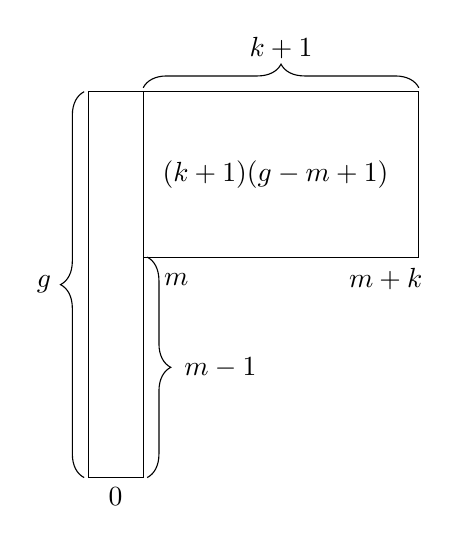
\begin{tikzpicture}[scale=1.4]
            \coordinate (A) at (0,0);
            \coordinate (B) at (0.5,2);
            \coordinate (C) at (0,3.5);
            \coordinate (D) at (0.5,0);
            \coordinate (E) at (0.5,3.5);
            \coordinate (F) at (3,2);
            \coordinate (G) at (3,3.5);
            \coordinate (H) at (0.23,1);

            \draw (A) -- (C);
            \draw (A) -- (D) node[midway, below] {$0$};
            \draw (D) -- (E);
            \draw (B) -- (E);
            \draw (B) -- (F);
            \draw (F) -- (G);
            \draw (G) -- (C);

            \node at (1.7,2.75) {$(k+1)(g-m+1)$};
            \node at (0.8,1.8) {$m$};
            \node at (2.7,1.8) {$m+k$};

            \draw[decorate,decoration={brace,amplitude=3mm, raise=0.5mm}] (A) -- (C);
            \draw[decorate,decoration={brace,amplitude=3mm, raise=0.5mm}] (B) -- (D);
            \draw[decorate,decoration={brace,amplitude=3mm, raise=0.5mm}] (E) -- (G);

            \node at (-0.4,1.75) {$g$};
            \node at (1.2,1) {$m-1$};
            \node at (1.75,3.9) {$k+1$};
        \end{tikzpicture}
        \end{center}
\end{frame}

\begin{frame}{Pflueger's Conjecture for NS of Depth 2}
    Thus, $ewt=(k+1)(g-m+1)$. Additionally, $F=g+(k+1).$ Since the numerical semigroup has depth 2, $m<g+k+1<2m$, or $k\leq 2m-g-2.$ So, \[(2m-g-1)(g-m+1)=-2(m-1)^2 + (3g - 1)(m - 1) - (g^2 - g)\] is the largest effective weight. Optimizing this function with respect to $m$, we get that the maximum of the function is 
    \[\frac{(g+1)^2}{8}\]
    at $m=\ds\frac{3(g+1)}{4}$.
\end{frame}

\begin{frame}{What about NS of higher depths?}
    But this geometric approach is significantly more complicated when we consider numerical semigroups of larger depths. We introduce Apery tuples which will help us prove the conjecture for numerical semigroups of higher depths.
\end{frame}

\begin{frame}{Apery Set}

Let $S$ be a numerical semigroup and $n\in S-\{0\}$. We define the \textbf{Apery set} with respect to $n$ to be 
\[\Ap(S,n)=\{s\in S:s-n\notin S\}.\] We denote $\Ap(S)$ as the Apery set with respect to $m(S)$, i.e.
\[\Ap(S)=\{s\in S:s-m(S)\notin S\}.\]

\textbf{NOTE:} By this definition, $\Ap(S)$ contains exactly one element of $S$ from each congruence class modulo $m(S)$.
\end{frame}

\begin{frame}{Apery Set}
    \[S=\{0,4,6,8,9,10,12,13,14,15,\to\}\]
    \begin{center}
    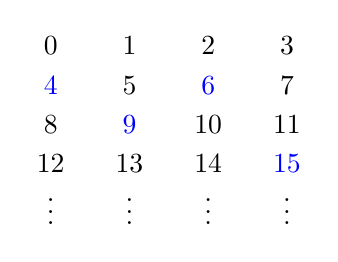
\begin{tikzpicture}
        \node at (0.5, 2) {$0$}; 
        \node at (1.5, 2) {$1$}; 
        \node at (2.5, 2) {$2$}; 
        \node at (3.5, 2) {$3$}; 
        \node at (0.5, 1.5) {\textcolor{blue}{$4$}}; 
        \node at (1.5, 1.5) {$5$}; 
        \node at (2.5, 1.5) {\textcolor{blue}{$6$}}; 
        \node at (3.5, 1.5) {$7$}; 
        \node at (0.5, 1) {$8$}; 
        \node at (1.5, 1) {\textcolor{blue}{$9$}}; 
        \node at (2.5, 1) {$10$}; 
        \node at (3.5, 1) {$11$}; 
        \node at (0.5, 0.5) {$12$}; 
        \node at (1.5, 0.5) {$13$}; 
        \node at (2.5, 0.5) {$14$}; 
        \node at (3.5, 0.5) {\textcolor{blue}{$15$}}; 
        \node at (0.5, 0) {\vdots}; 
        \node at (1.5, 0) {\vdots}; 
        \node at (2.5, 0) {\vdots}; 
        \node at (3.5, 0) {\vdots};
    \end{tikzpicture}
    \end{center}\vspace{8pt}
    Apery set of $S$ is 
    \begin{align*}
        \Ap(S,4)&=\{0,9,6,15\}\\
                &=\{0,2\cdot 4+1,1\cdot 4+2,3\cdot 4+3\}
    \end{align*}
\end{frame}

\begin{frame}{Apery tuple/Kunz coordinate vector}

\[S=\{0,4,6,8,9,10,12,13,14,15,\to\}\]
\begin{center}
    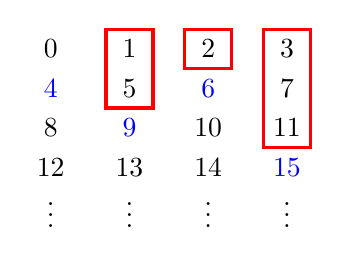
\begin{tikzpicture}
        \node at (0.5, 2) {$0$}; 
        \node at (1.5, 2) {$1$}; 
        \node at (2.5, 2) {$2$}; 
        \node at (3.5, 2) {$3$}; 
        \node at (0.5, 1.5) {\textcolor{blue}{$4$}}; 
        \node at (1.5, 1.5) {$5$}; 
        \node at (2.5, 1.5) {\textcolor{blue}{$6$}}; 
        \node at (3.5, 1.5) {$7$}; 
        \node at (0.5, 1) {$8$}; 
        \node at (1.5, 1) {\textcolor{blue}{$9$}}; 
        \node at (2.5, 1) {$10$}; 
        \node at (3.5, 1) {$11$}; 
        \node at (0.5, 0.5) {$12$}; 
        \node at (1.5, 0.5) {$13$}; 
        \node at (2.5, 0.5) {$14$}; 
        \node at (3.5, 0.5) {\textcolor{blue}{$15$}}; 
        \node at (0.5, 0) {\vdots}; 
        \node at (1.5, 0) {\vdots}; 
        \node at (2.5, 0) {\vdots}; 
        \node at (3.5, 0) {\vdots};

    \draw[red, very thick] (1.2,1.25) rectangle (1.8,2.25);
    \draw[red, very thick] (2.2,1.75) rectangle (2.8,2.25);
    \draw[red, very thick] (3.2,0.75) rectangle (3.8,2.25);

    \end{tikzpicture}
\end{center}

    The Apery set of $S$ is 
    \begin{align*}
        \Ap(S,4)&=\{0,9,6,15\}\\
                &=\{0,\textcolor{red}{2}\cdot 4+1,\textcolor{red}{1}\cdot 4+2,\textcolor{red}{3}\cdot 4+3\}
    \end{align*}

    The Apery tuple (or Kunz coordinate vector) of $S$ is 
    \[\KC(S,4)=(\textcolor{red}{2},\textcolor{red}{1},\textcolor{red}{3})\]
    
\end{frame}

\begin{frame}
    Notice that the $S=\langle 4,6,9\rangle$. In other words, $4,6,9$ generate $S$. In fact, they are the minimal generators of $S$. Additionally, if we swap out our class representative (remove 0, add 4), our minimal generators are all elements of the Apery set. This is indeed always the case.
\end{frame}

\begin{frame}{Apery Weight}
    Now, we define the \textbf{Apery weight} of a numerical semigroup $S$, denoted by $\Apwt(S)$, as
    \[\sum_{x\in S} \#\{\text{gaps above}\; x\}\quad\text{where}\; x\;\text{is $m(S)$ or a nonzero Apery element}\]
    \vspace{1cm}
    
    \textbf{NOTE:} Since all minimal generators are elements of the Apery set, the Apery weight is an upper bound for the effective weight.
\end{frame}

\begin{frame}{Pflueger's Conjecture for NS of Depth 3 (kind of)}
    Consider a numerical semigroup, $S$, of depth 3. Then, the Apery tuple of $S$ contains only 1s, 2s, and 3s. Suppose the Apery tuple of $S$ is of the form 
    \[(\underbrace{1,\dots,1}_{x},\underbrace{2,\dots,2}_{y},\underbrace{3,\dots,3}_{z})\]
We are able to show that
    \[\Apwt(S)=(g-(m-1))+2xz+yz+xy.\]
Since 
\[g=x+2y+3z\quad\text{ and }\quad m-1=x+y+z,\]
we find that $\Apwt(S)=\frac{g^2}{9}+\frac{g}{3}+\frac{1}{4}\leq \left\lfloor\frac{(g+1)^2}{8} \right\rfloor$
\end{frame}

\begin{frame}{Further Work}
    \begin{itemize}
        \item Dropping the ascending order condition
        \item Generalizing to NS of all depths
    \end{itemize}
\end{frame}

\begin{frame}{Fun Connection to Algebraic Geometry}
Pflueger's interest in effective weight comes from the fact that it provides an upper bound for the codimension of the space of algebraic curves with a marked point and a given Weierstrass point inside the moduli space of genus g curves with one marked point.
\end{frame}

\section{Acknowledgments}
\begin{frame}{Acknowledgments}
Thank you to everyone on my team, including my fellow undergraduate researchers, our graduate student advisors, and our faculty advisor, Dr. Nathan Kaplan! Thank you to Cal-Bridge for their generous funding!
\begin{columns}[c]
            \begin{column}{.25\textwidth}
            \begin{figure}
                \centering
                \includegraphics[width=1\textwidth]{Victoria/Logos/CSU,Fresno.png}
            \end{figure}      
            \end{column}
            \begin{column}{.25\textwidth}
            \begin{figure}
                \centering
                \includegraphics[width=1.2\textwidth]{Victoria/Logos/Cal-Bridge.jpg}
            \end{figure}
            \end{column}
            \begin{column}{.25\textwidth}
            \begin{figure}
                \centering
                \includegraphics[width=1\textwidth]{Victoria/Logos/UC, Irvine.png}
            \end{figure}
            \end{column}
        \end{columns}

\end{frame}

\end{document}
